\section{Streaming video}
\label{sec:attend_the_course}

Through the platform of e-learning, the student will find their own course of interest selecting it from those available.
The user chosen and eventually paid the course,then he can start his training.
Also for streaming it has created a web component that allows the video vision, hiding all  encountered problems on the thesis work and complexity that shown in chapter 3.

\begin{lstlisting}[language=html]
       <deck-video src="{{data.lecture.video.url}}"></deck-video>
\end{lstlisting}

The final result will be a player to stream video content as you can see in the picture

\begin{figure}[htb]
 \centering
 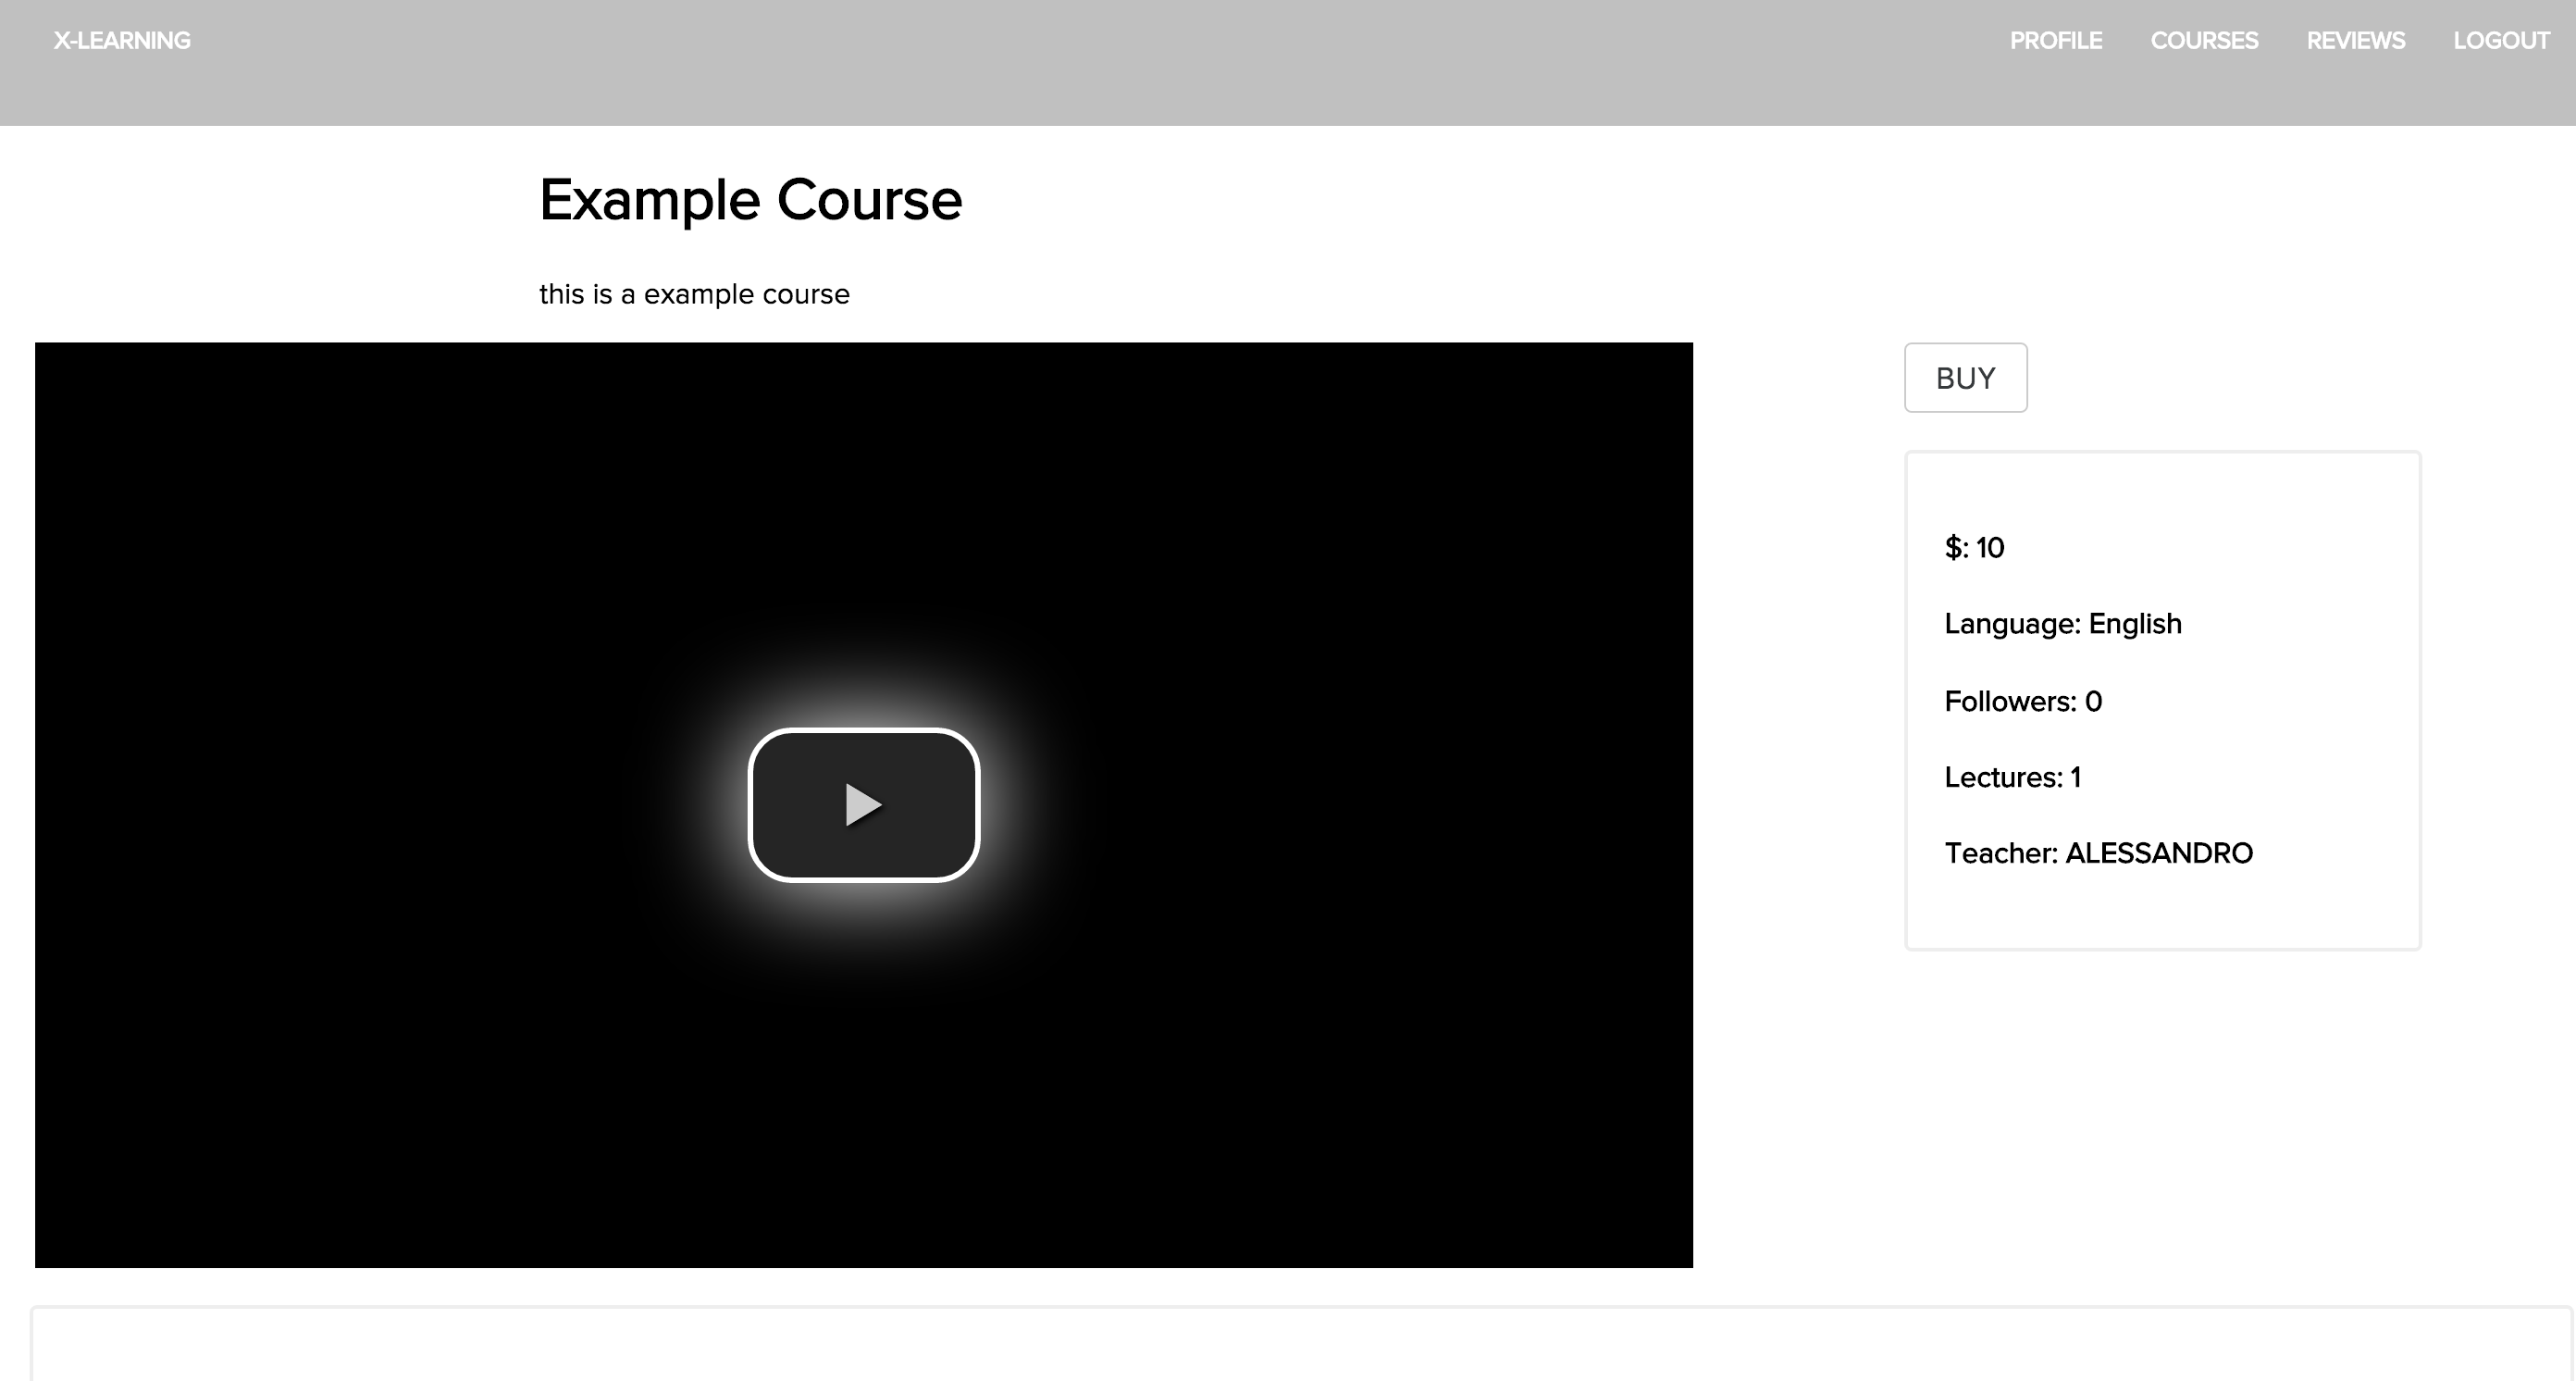
\includegraphics[width=1.0\linewidth]{images/chapter6/deck_video.png}\hfill
 \caption[Deck video]{Deck video}
 \label{fig:fourV}
\end{figure}
